\question[7] Consider the non-linear system below.  
\begin{align*}
    \dxdt &= (x-1)(y-1) , \qquad \dydt = y+x^2-5
\end{align*}
\begin{parts}
\part Sketch the nullclines of the system on the axes below. Clearly indicate the critical points.
    \ifnum \Solutions=1 {\color{DarkBlue} \\[12pt] 
    Green curves are the $x-$nullclines, black curves are the $y-$nullclines.
    \begin{center}
    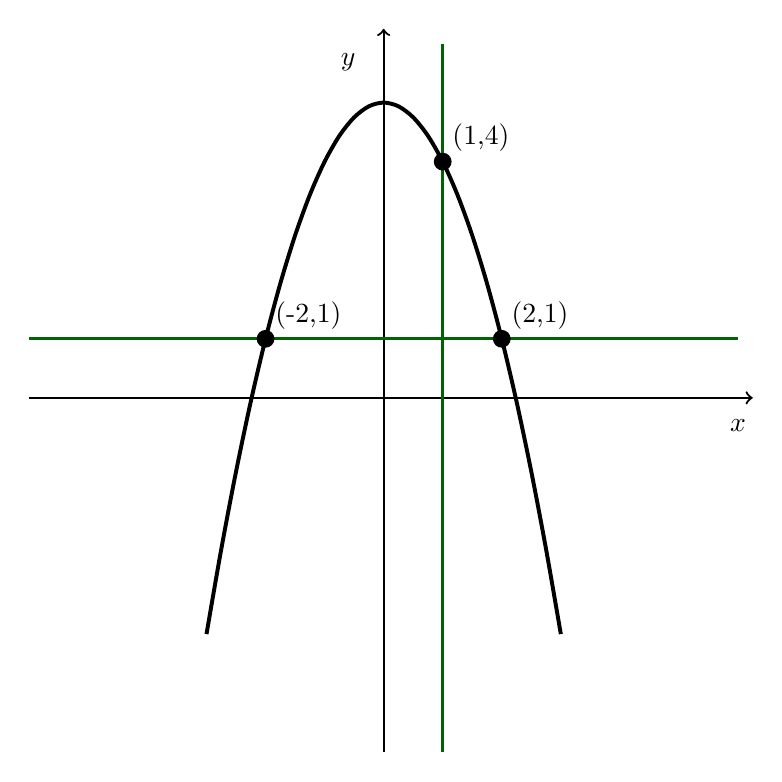
\begin{tikzpicture}[scale=0.75]
    \draw[thick, ->] (-6, 0) -- (6.25, 0);
    \draw[thick, ->] (0, -6) -- (0, 6.25);
    \node[overlay, below] at (6, -0.2) {$x$};
    \node[overlay, below] at (-0.6, 6) {$y$};   
    \draw[very thick,DarkGreen, -] (1, 6) -- (1, -6);        
    \draw[very thick,DarkGreen, -] (-6, 1) -- (6, 1);   
    \draw[black, line width = 0.50mm]   plot[smooth,domain=-3:3] (\x, {5-\x*\x});
    \filldraw[black] (1,4) circle (4pt) node[anchor=south west]{(1,4)};
    \filldraw[black] (2,1) circle (4pt) node[anchor=south west]{(2,1)};
    \filldraw[black] (-2,1) circle (4pt) node[anchor=south west]{(-2,1)};
    \end{tikzpicture}
    \end{center}            
    } 
    \else 
    \begin{center}
    \begin{tikzpicture}[scale=0.55]
    \draw[very thick, ->] (-6, 0) -- (6.25, 0);
    \draw[very thick, ->] (0, -6) -- (0, 6.25);
    \node[overlay, below] at (6, -0.2) {$x$};
    \node[overlay, below] at (-0.6, 6) {$y$};        
    \end{tikzpicture}
    \end{center}    
    \fi
    \part Determine the locations of the critical points. 
    \ifnum \Solutions=1 {\color{DarkBlue} \\[12pt] 
    Setting both $x'=0$ and $y'=0$, we obtain three critical points as follows. 
    
    Setting $x'=0$ implies $y=1$ or $x=1$. 
        \begin{itemize}
            \item If $y=1$, then for $y'=0$ we need $x=\pm2$. There are CPs at $(-2,1)$ and $(2,1)$. 
            \item If $x=0$, then for $y'=0$ we solve $0 = y + 1^2 - 5$. So there is a CP at $(1,4)$.
        \end{itemize}
        The CPs are located at $(1,4)$, $(-2,1)$, $(2,1)$. 
        } 
    \else 
    \vfill
    \fi
\end{parts}
